\chapter{Zadatak 1c --- grafički prikaz}
\label{ch:z1-graficki}

\section{Što se ovdje traži}

Četiri stvari na jednoj slici: dopustivi skup, nivo-krivulje funkcije cilja,
izračunati gradijenti i njihova skica u KKT točki. I --- što zadatak ne kaže
izrijekom, ali se očekuje --- objašnjenje što se s te slike vidi.

\begin{zadatak}{Zadatak 1, podzadatak c)}
c) Nacrtajte dozvoljeni skup, nivo krivulje funkcije cilja te izračunajte i
skicirati gradijente ograničenja i funkcije cilja u točki koja zadovoljava KKT
uvjete.
\end{zadatak}

\begin{predznanje}
\begin{itemize}[nosep,leftmargin=*]
  \item Što je nivo-krivulja i zašto su ovdje elipse --- \S\ref{sec:nivo-krivulje}.
  \item Gradijent je okomit na nivo-krivulju --- \S\ref{sec:gradijent-na-slici}.
  \item Crtanje poluprostora iz nejednakosti --- \S\ref{sec:poluprostor}.
  \item Rješenje $\xopt$ i $\muopt$ --- \eqref{eq:z1b-rjesenje}.
\end{itemize}
\end{predznanje}

\section{Gradijenti u KKT točki}
\label{sec:z1c-gradijenti}

\begin{korak}[Izračun triju gradijenata]
\begin{enumerate}[leftmargin=*]
  \item \textbf{Gradijent funkcije cilja.} Iz $\grad f(x) = Qx + c$ uz
        $\xopt = (190/33,\; 140/33)$:
        \[
          \grad f(\xopt) =
          \begin{bmatrix} 2\cdot\frac{190}{33} - 0{,}3\cdot\frac{140}{33} + 2 \\[4pt]
                          -0{,}3\cdot\frac{190}{33} + 4\cdot\frac{140}{33} - 3 \end{bmatrix}
          = \begin{bmatrix} \frac{404}{33} \\[4pt] \frac{404}{33} \end{bmatrix}
          = \begin{bmatrix} 12{,}242424 \\ 12{,}242424 \end{bmatrix}.
        \]
        Provjera druge komponente:
        $-57/33 + 560/33 - 99/33 = 404/33$. \checkmark
  \item \textbf{Gradijent prvog ograničenja.} $g_1$ je afina, pa je gradijent
        konstantan: $\grad g_1 = \begin{bsmallmatrix} -1 \\ -1 \end{bsmallmatrix}$.
  \item \textbf{Gradijent drugog ograničenja.}
        $\grad g_2 = \begin{bsmallmatrix} 1 \\ -1 \end{bsmallmatrix}$, također
        konstantan.
\end{enumerate}
\end{korak}

\begin{formula}{Uvjet stacionarnosti, provjeren brojevima}
\begin{equation}
\grad f(\xopt) = -\mu_1^{\star}\,\grad g_1(\xopt)
= -\frac{404}{33}\begin{bmatrix} -1 \\ -1 \end{bmatrix}
= \begin{bmatrix} 12{,}242424 \\ 12{,}242424 \end{bmatrix} . \quad\checkmark
\label{eq:z1c-kolinearnost}
\end{equation}
Gradijent funkcije cilja i gradijent aktivnog ograničenja su \textbf{kolinearni i
suprotno usmjereni}. Ograničenje $g_2$ je neaktivno, $\mu_2^{\star} = 0$, pa
njegov gradijent u ravnotežu uopće ne ulazi.
\end{formula}

To da je $\grad f(\xopt)$ ispao s objema komponentama jednakima nije slučajnost:
ograničenje $g_1$ ima gradijent $(-1,-1)$, a stacionarnost traži da $\grad f$
bude njegov negativni višekratnik --- dakle nužno oblika $(\alpha, \alpha)$.

\section{Slika iz seminara i njezino čitanje}
\label{sec:z1c-slika}

\begin{figure}[H]
\centering
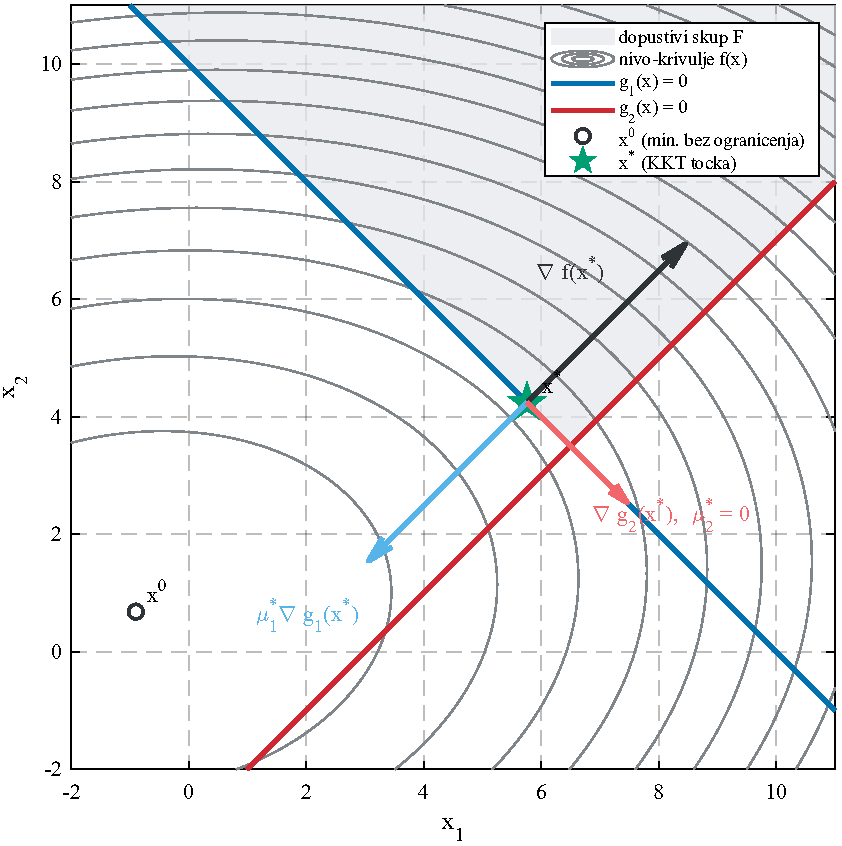
\includegraphics[width=0.92\linewidth]{../figures/fig1_1_qp_primal_geometry.pdf}
\caption{Dopustivi skup, nivo-krivulje funkcije cilja i gradijenti u KKT točki
$\xopt$ (Slika 2.1 seminara v1.2). Duljine vektora grafički su skalirane.}
\label{fig:z1c-geometrija}
\end{figure}

\subsection{Dekonstrukcija: svaki element slike posebno}

\begin{longtable}{@{}p{0.30\linewidth} p{0.66\linewidth}@{}}
\toprule
\textbf{Element} & \textbf{Što je i odakle dolazi} \\
\midrule
\endfirsthead
\toprule
\textbf{Element} & \textbf{Što je i odakle dolazi} \\
\midrule
\endhead
Osi $x_1$, $x_2$ & Prostor projektnih varijabli. Raspon je otprilike $-2$ do $11$
po obje osi, tek toliko da stanu i neograničeni minimum i KKT točka. \\[5pt]
Puna debela crta & Rub prvog ograničenja, $g_1(x) = 0$, tj.\ pravac
$x_1 + x_2 = 10$. Ide od gore lijevo prema dolje desno. \\[5pt]
Crtkano-točkasta crta & Rub drugog ograničenja, $g_2(x) = 0$, tj.\ pravac
$x_1 - x_2 = 3$. Ide od dolje lijevo prema gore desno. \\[5pt]
Sivo osjenčano područje & Dopustivi skup $\feas$: presjek poluprostora
$x_1 + x_2 \geq 10$ i $x_1 - x_2 \leq 3$. Klin koji se otvara prema gore desno,
s vrhom u $(6{,}5,\; 3{,}5)$. Neograničen je. \\[5pt]
Tanke koncentrične krivulje & Nivo-krivulje funkcije cilja. Elipse su jer je
$Q \pd 0$; središte im je u $x^{0}$, blago su nagnute i rastu prema van. \\[5pt]
Kružić, oznaka $x^{0}$ & Minimum bez ograničenja,
$x^{0} = (-0{,}898,\; 0{,}683)$. Leži \emph{izvan} sive površine --- to je
vizualni dokaz da Slučaj 1 otpada. \\[5pt]
Zvjezdica, oznaka $\xopt$ & KKT točka $(5{,}758,\; 4{,}242)$. Leži \emph{na}
punoj crti, dakle na rubu $g_1$, i to gore lijevo od vrha klina. \\[5pt]
Crna strelica iz $\xopt$ prema gore desno & $\grad f(\xopt)$, smjer $(1,1)$.
Pokazuje u smjeru rasta cilja, dakle u unutrašnjost dopustivog skupa. \\[5pt]
Siva strelica iz $\xopt$ prema dolje lijevo & $\mu_1^{\star}\grad g_1(\xopt)$,
smjer $(-1,-1)$. Točno suprotna prethodnoj --- to je slika jednadžbe
\eqref{eq:z1c-kolinearnost}. \\[5pt]
Kratka strelica desno od $\xopt$, uz oznaku $\mu_2^{\star} = 0$ & $\grad g_2$,
smjer $(1,-1)$. Nacrtana je da se vidi da postoji, ali s množiteljem nula ne
sudjeluje u ravnoteži. \\
\bottomrule
\end{longtable}

\subsection{Što slika dokazuje}

\begin{korak}[Tri zaključka koja se čitaju izravno s crteža]
\begin{enumerate}[leftmargin=*]
  \item \textbf{Zašto optimum nije $x^{0}$.} Kružić $x^{0}$ je izvan sive
        površine. Neograničeni minimum nije dopustiv, pa se rješenje mora
        pomaknuti na rub.
  \item \textbf{Zašto je optimum baš tu, a ne u vrhu.} Nivo-elipsa koja prolazi
        kroz $\xopt$ \emph{dodiruje} punu crtu --- tangentna je na nju. Kroz vrh
        $(6{,}5,\, 3{,}5)$ prolazi elipsa \emph{veće} razine, koja rub siječe. Da
        siječe, postojao bi pomak uzduž ruba koji ostaje dopustiv i smanjuje
        cilj; upravo taj pomak vodi od vrha do $\xopt$.
  \item \textbf{Zašto su KKT uvjeti zadovoljeni.} Dvije glavne strelice leže na
        istom pravcu i suprotno su usmjerene. To je geometrijski oblik uvjeta
        $\grad f + \mu_1 \grad g_1 = 0$. Kad bi među njima bio kut različit od
        $180^\circ$, postojala bi komponenta gradijenta cilja uzduž ruba --- a
        onda bi se klizanjem uzduž ruba cilj mogao smanjiti.
\end{enumerate}
\end{korak}

\section{Kako sliku nacrtati rukom}
\label{sec:z1c-crtanje}

\begin{ploca}[Cijela slika Zadatka 1c, deset poteza]
\begin{enumerate}[leftmargin=*]
  \item \textbf{Osi.} Vodoravna $x_1$, okomita $x_2$. Označi brojeve $0$, $5$,
        $10$ na objema. Ostavi malo prostora lijevo od nule, jer ondje ide $x^{0}$.
  \item \textbf{Prvi pravac.} $x_1 + x_2 = 10$ kroz $(10,0)$ i $(0,10)$. Povuci
        ga \emph{debelo} --- to je aktivno ograničenje.
  \item \textbf{Drugi pravac.} $x_1 - x_2 = 3$ kroz $(3,0)$ i $(6{,}5,\, 3{,}5)$.
        Povuci ga crtkano.
  \item \textbf{Vrh.} Označi sjecište $(6{,}5,\; 3{,}5)$ i napiši mu koordinate.
  \item \textbf{Dopustiva strana.} Uvrsti ishodište: $g_1(0,0) = 10 > 0$ (nije
        dopustivo), $g_2(0,0) = -3 < 0$ (dopustivo). Osjenčaj klin koji se otvara
        gore desno, od vrha prema gore.
  \item \textbf{Središte elipsa.} Ucrtaj kružić u $(-0{,}9,\; 0{,}7)$ i označi
        ga $x^{0}$. Izgovori: ,,neograničeni minimum, nije dopustiv``.
  \item \textbf{Elipse.} Tri koncentrične elipse oko $x^{0}$, blago nagnute
        (oko $8^\circ$), sve veće prema van. Najveću povuci tako da \emph{dodirne}
        debeli pravac.
  \item \textbf{KKT točka.} Točka dodira te elipse i debelog pravca je $\xopt$.
        Označi je zvjezdicom i napiši $(5{,}76,\; 4{,}24)$. Naglasi da je lijevo
        od vrha.
  \item \textbf{Dvije glavne strelice.} Iz $\xopt$ jedna strelica pod
        $45^\circ$ gore desno --- to je $\grad f(\xopt)$; i jedna jednako duga
        točno suprotno, dolje lijevo --- to je $\mu_1^{\star}\grad g_1$. Obje su
        okomite na debeli pravac.
  \item \textbf{Treća strelica.} Kratka strelica u smjeru $(1,-1)$, dolje desno,
        označena $\grad g_2$, uz napomenu $\mu_2^{\star} = 0$.
\end{enumerate}
\end{ploca}

\begin{zamka}[Zamka: elipsa koja siječe umjesto da dodiruje]
Ako na ploči nacrtaš elipsu koja \emph{siječe} rub u dvije točke, sam si sebi
nacrtao proturječje --- takva slika kaže da postoji dopustiv pomak koji smanjuje
cilj. Elipsa kroz optimum mora rub dodirivati u točno jednoj točki. Ako ti se pri
crtanju to ne uspije pogoditi, reci naglas: ,,skica nije u mjerilu, ali ključno
je da je u optimumu nivo-krivulja tangentna na aktivno ograničenje``.
\end{zamka}

\begin{zamka}[Zamka: smjer gradijenta cilja]
$\grad f(\xopt)$ pokazuje \emph{u} dopustivi skup, ne iz njega. Razlog: funkcija
cilja u tom smjeru raste, a dopustivi skup se prostire prema gore desno. Ono što
pokazuje van jest $-\grad f(\xopt)$, smjer najbržeg pada --- i baš zato optimum
i jest optimum: jedini smjer u kojem bi se cilj smanjio vodi izvan dopustivog
skupa.
\end{zamka}

\section{Kako je to riješeno u seminaru}
\label{sec:z1c-seminar}

\begin{seminar}{Seminar v1.2, §2.4 --- ,,(c) Grafički prikaz``}
U KKT točki $x^*$ gradijenti funkcije cilja i funkcija ograničenja iznose
\[
\nabla f(x^*) = Q x^* + c = \begin{bmatrix} 12.242424 \\ 12.242424 \end{bmatrix}, \quad
\nabla g_1(x^*) = \begin{bmatrix} -1 \\ -1 \end{bmatrix}, \quad
\nabla g_2(x^*) = \begin{bmatrix} 1 \\ -1 \end{bmatrix},
\]
pa uvjet stacionarnosti $(\star)$ daje
\[
\nabla f(x^*) = -\mu_1^* \nabla g_1(x^*) = -\frac{404}{33} \begin{bmatrix} -1 \\ -1 \end{bmatrix}.
\]
Gradijent funkcije cilja i gradijent aktivnog ograničenja su kolinearni i
suprotnog smjera. Ograničenje $g_2$ je neaktivno ($g_2(x^*) = -1.484848 < 0$), pa
je iz $(\star\star)$ $\mu_2^* = 0$ i njegov gradijent ne ulazi u ravnotežu.

Slika 2.1 prikazuje dopustivi skup $\mathcal{F}$ (osjenčano), nivo-krivulje
funkcije cilja, minimum bez ograničenja $x^0$ i KKT točku $x^*$ s ucrtanim
gradijentima. Nivo-krivulje su elipse jer je $Q \succ 0$. Duljine vektora na
slici su grafički skalirane.
\end{seminar}

Slika je izrađena u MATLAB-u; provjera kolinearnosti ispisana je u
\texttt{docs/code/task1\_output.txt}:

\begin{lstlisting}[style=outputstyle]
grad f(x*) = [12.242424, 12.242424];  -mu1*grad g1 = [12.242424, 12.242424]
\end{lstlisting}

\section{Modelski odgovori}
\label{sec:z1c-odgovori}

\begin{pitanje}{Zašto su nivo-krivulje elipse, a ne kružnice?}
\textbf{Odgovor.} Bile bi kružnice samo da je $Q$ višekratnik jedinične matrice,
dakle da su obje svojstvene vrijednosti jednake. Ovdje su $1{,}956$ i $4{,}044$,
pa je omjer poluosi $\sqrt{4{,}044/1{,}956} \approx 1{,}44$, a osi su zakrenute
za oko $8^\circ$ jer svojstveni vektori nisu poklopljeni s koordinatnim osima ---
posljedica mješovitog člana $-0{,}3\,x_1x_2$.
\end{pitanje}

\begin{pitanje}{Što biste vidjeli na slici da je $\mu_2^{\star} > 0$?}
\textbf{Odgovor.} Optimum bi bio u vrhu klina, a $-\grad f$ bi ležao \emph{unutar}
stošca razapetog s $\grad g_1$ i $\grad g_2$, dakle bio bi njihova kombinacija s
oba pozitivna koeficijenta. Kod nas $-\grad f$ leži točno na bridu tog stošca,
uzduž $\grad g_1$, pa je drugi koeficijent nula.
\end{pitanje}

\begin{pitanje}{Kako biste sa slike provjerili da je rješenje globalno, a ne lokalno?}
\textbf{Odgovor.} Sa same slike ne bih --- globalnost ne slijedi iz crteža nego
iz konveksnosti. Slika pokazuje da je uvjet stacionarnosti zadovoljen; da je taj
uvjet i \emph{dovoljan} slijedi iz toga što je problem konveksan i što je
Slaterov uvjet zadovoljen. Slika je ilustracija, ne dokaz.
\end{pitanje}

\begin{izgovor}[Čitanje slike naglas]
,,Na apscisi je $x_1$, na ordinati $x_2$. Osjenčano je dopustivo područje,
presjek poluprostora $x_1 + x_2 \geq 10$ i $x_1 - x_2 \leq 3$; to je neograničen
klin s vrhom u šest i pol, tri i pol.

Tanke koncentrične krivulje su nivo-krivulje funkcije cilja. Elipse su jer je
matrica ku pozitivno definitna, a središte im je u neograničenom minimumu minus
nula devet, nula šest osam --- koji je, kako se vidi, izvan dopustivog područja.

Zvjezdica je KKT točka, pet zarez sedam šest, četiri zarez dva četiri. Leži na
rubu prvog ograničenja, lijevo od vrha. Nivo-elipsa kroz nju tangentna je na taj
rub.

Iz te točke izlaze dvije strelice na istom pravcu i suprotnih smjerova:
gradijent funkcije cilja, koji pokazuje u dopustivo područje, i mi jedan puta
gradijent prvog ograničenja, koji pokazuje van. Njihov zbroj je nula --- to je
uvjet stacionarnosti, sada vidljiv na slici. Treća strelica je gradijent drugog
ograničenja; ono je neaktivno, množitelj mu je nula, pa u ravnotežu ne ulazi.
Duljine strelica su skalirane radi preglednosti, uspoređujem samo smjerove.``
\end{izgovor}
